\documentclass[12pt]{article}
\usepackage[left=1cm, right=1cm, top=2cm,bottom=1.5cm]{geometry} 

\usepackage[parfill]{parskip}
\usepackage[utf8]{inputenc}
\usepackage[T2A]{fontenc}
\usepackage[russian]{babel}
\usepackage{enumitem}
\usepackage[normalem]{ulem}
\usepackage{amsfonts, amsmath, amsthm, amssymb, mathtools,xcolor}
\usepackage{blkarray}

\usepackage{tabularx}
\usepackage{hhline}

\usepackage{accents}
\usepackage{fancyhdr}
\pagestyle{fancy}
\renewcommand{\headrulewidth}{1.5pt}
\renewcommand{\footrulewidth}{1pt}

\usepackage{graphicx}
\usepackage[figurename=Рис.]{caption}
\usepackage{subcaption}
\usepackage{float}

%%Наименование папки откуда забирать изображения
\graphicspath{ {./images/} }

%%Изменение формата для ввода доказательства
\renewcommand{\proofname}{$\square$  \nopunct}
\renewcommand\qedsymbol{$\blacksquare$}

%%Изменение отступа на таблицах
\addto\captionsrussian{%
	\renewcommand{\proofname}{$\square$ \nopunct}%
}
%% Римские цифры
\newcommand{\RN}[1]{%
	\textup{\uppercase\expandafter{\romannumeral#1}}%
}

%% Для удобства записи
\newcommand{\MR}{\mathbb{R}}
\newcommand{\MC}{\mathbb{C}}
\newcommand{\MQ}{\mathbb{Q}}
\newcommand{\MN}{\mathbb{N}}
\newcommand{\MZ}{\mathbb{Z}}
\newcommand{\MTB}{\mathbb{T}}
\newcommand{\MTI}{\mathbb{I}}
\newcommand{\MI}{\mathrm{I}}
\newcommand{\MCI}{\mathcal{I}}
\newcommand{\MJ}{\mathrm{J}}
\newcommand{\MH}{\mathrm{H}}
\newcommand{\MT}{\mathrm{T}}
\newcommand{\MU}{\mathcal{U}}
\newcommand{\MV}{\mathcal{V}}
\newcommand{\MB}{\mathcal{B}}
\newcommand{\MF}{\mathcal{F}}
\newcommand{\MW}{\mathcal{W}}
\newcommand{\ML}{\mathcal{L}}
\newcommand{\MP}{\mathcal{P}}
\newcommand{\VN}{\varnothing}
\newcommand{\VE}{\varepsilon}
\newcommand{\dx}{\, dx}
\newcommand{\dy}{\, dy}
\newcommand{\dz}{\, dz}
\newcommand{\dd}{\, d}


\theoremstyle{definition}
\newtheorem{defn}{Опр:}
\newtheorem{rem}{Rm:}
\newtheorem{prop}{Утв.}
\newtheorem{exrc}{Упр.}
\newtheorem{problem}{Задача}
\newtheorem{lemma}{Лемма}
\newtheorem{theorem}{Теорема}
\newtheorem{corollary}{Следствие}

\newenvironment{cusdefn}[1]
{\renewcommand\thedefn{#1}\defn}
{\enddefn}

\DeclareRobustCommand{\divby}{%
	\mathrel{\text{\vbox{\baselineskip.65ex\lineskiplimit0pt\hbox{.}\hbox{.}\hbox{.}}}}%
}
\DeclareRobustCommand{\ndivby}{\mkern-1mu\not\mathrel{\mkern4.5mu\divby}\mkern1mu}


%Короткий минус
\DeclareMathSymbol{\SMN}{\mathbin}{AMSa}{"39}
%Длинная шапка
\newcommand{\overbar}[1]{\mkern 1.5mu\overline{\mkern-1.5mu#1\mkern-1.5mu}\mkern 1.5mu}
%Функция знака
\DeclareMathOperator{\sgn}{sgn}

%Функция ранга
\DeclareMathOperator{\rk}{\text{rk}}
\DeclareMathOperator{\diam}{\text{diam}}


%Обозначение константы
\DeclareMathOperator{\const}{\text{const}}

\DeclareMathOperator{\codim}{\text{codim}}

\DeclareMathOperator*{\dsum}{\displaystyle\sum}
\newcommand{\ddsum}[2]{\displaystyle\sum\limits_{#1}^{#2}}

%Интеграл в большом формате
\DeclareMathOperator{\dint}{\displaystyle\int}
\newcommand{\ddint}[2]{\displaystyle\int\limits_{#1}^{#2}}
\newcommand{\ssum}[1]{\displaystyle \sum\limits_{n=1}^{\infty}{#1}_n}

\newcommand{\smallerrel}[1]{\mathrel{\mathpalette\smallerrelaux{#1}}}
\newcommand{\smallerrelaux}[2]{\raisebox{.1ex}{\scalebox{.75}{$#1#2$}}}

\newcommand{\smallin}{\smallerrel{\in}}
\newcommand{\smallnotin}{\smallerrel{\notin}}

\newcommand*{\medcap}{\mathbin{\scalebox{1.25}{\ensuremath{\cap}}}}%
\newcommand*{\medcup}{\mathbin{\scalebox{1.25}{\ensuremath{\cup}}}}%

\makeatletter
\newcommand{\vast}{\bBigg@{3.5}}
\newcommand{\Vast}{\bBigg@{5}}
\makeatother

%Промежуточное значение для sup\inf, поскольку они имеют разную высоту
\newcommand{\newsup}{\mathop{\smash{\mathrm{sup}}}}
\newcommand{\newinf}{\mathop{\mathrm{inf}\vphantom{\mathrm{sup}}}}

%Скалярное произведение
\newcommand{\inner}[2]{\left\langle #1, #2 \right\rangle }
\newcommand{\linsp}[1]{\left\langle #1 \right\rangle }
\newcommand{\linmer}[2]{\left\langle #1 \vert #2\right\rangle }

%Подпись символов снизу
\newcommand{\ubar}[1]{\underaccent{\bar}{#1}}

%% Шапка для букв сверху
\newcommand{\wte}[1]{\widetilde{#1}}
\newcommand{\wht}[1]{\widehat{#1}}
\newcommand{\ovl}[1]{\overline{#1}}

%%Трансформация Фурье
\newcommand{\fourt}[1]{\mathcal{F}\left(#1\right)}
\newcommand{\ifourt}[1]{\mathcal{F}^{-1}\left(#1\right)}

%%Символ вектора
\newcommand{\vecm}[1]{\overrightarrow{#1\,}}

%%Пространстов матриц
\newcommand{\matsq}[1]{\operatorname{Mat}_{#1}}
\newcommand{\mat}[2]{\operatorname{Mat}_{#1, #2}}

%Оператор для действ и мнимых чисел
\DeclareMathOperator{\IM}{\operatorname{Im}}
\DeclareMathOperator{\RE}{\operatorname{Re}}
\DeclareMathOperator{\li}{\operatorname{li}}
\DeclareMathOperator{\GL}{\operatorname{GL}}
\DeclareMathOperator{\SL}{\operatorname{SL}}
\DeclareMathOperator{\Char}{\operatorname{char}}

%Делимость чисел
\newcommand{\modn}[3]{#1 \equiv #2 \; (\bmod \; #3)}


%%Взятие в скобки, модули и норму
\newcommand{\parfit}[1]{\left( #1 \right)}
\newcommand{\modfit}[1]{\left| #1 \right|}
\newcommand{\sqparfit}[1]{\left\{ #1 \right\}}
\newcommand{\normfit}[1]{\left\| #1 \right\|}

%%Функция для обозначения равномерной сходимости по множеству
\newcommand{\uconv}[1]{\overset{#1}{\rightrightarrows}}
\newcommand{\uconvm}[2]{\overset{#1}{\underset{#2}{\rightrightarrows}}}


%%Функция для обозначения нижнего и верхнего интегралов
\def\upint{\mathchoice%
	{\mkern13mu\overline{\vphantom{\intop}\mkern7mu}\mkern-20mu}%
	{\mkern7mu\overline{\vphantom{\intop}\mkern7mu}\mkern-14mu}%
	{\mkern7mu\overline{\vphantom{\intop}\mkern7mu}\mkern-14mu}%
	{\mkern7mu\overline{\vphantom{\intop}\mkern7mu}\mkern-14mu}%
	\int}
\def\lowint{\mkern3mu\underline{\vphantom{\intop}\mkern7mu}\mkern-10mu\int}

%%След матрицы
\DeclareMathOperator*{\tr}{tr}

\makeatletter
\renewcommand*\env@matrix[1][*\c@MaxMatrixCols c]{%
	\hskip -\arraycolsep
	\let\@ifnextchar\new@ifnextchar
	\array{#1}}
\makeatother


%% Переопределение функции хи, чтобы выглядела более приятно
\makeatletter
\@ifdefinable\@latex@chi{\let\@latex@chi\chi}
\renewcommand*\chi{{\@latex@chi\smash[t]{\mathstrut}}} % want only bottom half of \mathstrut
\makeatletter

\begin{document}
\lhead{Алгебра-\RN{1}}
\chead{Тимашев Д.А.}
\rhead{Лекция - 13}
\section*{Изоморфизм}
\subsection*{Мотивация для изоморфизма}
Ещё раз вспомним аксиоматическое определение поля комплексных чисел.
\begin{defn}
	\uwave{Полем комплексных чисел} называется поле $\MC$, обладающее следующими свойствами:
	\begin{enumerate}[label=\arabic*)]
		\item $\MR \subset \MC$;
		\item $i \in \MC \colon i^2 = -1$, этот элемент называется \uwave{мнимой единицей};
		\item \textbf{Условие минимальности}: Если $K$ - подполе: $\MR \subseteq K \subseteq \MC, \, i \in K \Rightarrow K = \MC$;
	\end{enumerate}
\end{defn}
Пока остаются открытыми вопросы: существует ли поле комплексных чисел и если существует, то оно одно такое или их много? Начнем с вопроса единственности. Могут ли быть единственными математические структуры, которые определены аксиоматически своими свойствами? 

Пусть у нас есть поле $\MC$, удовлетворяющее свойствам из определения выше. Все элементы кроме тех, что в $\MR$ взаимнооднозначно заменим на элементы какого-то другого множества. Например:
$$
	\forall z \in \MC \setminus \MR, \, z \mapsto (z,z) \Rightarrow \MC \mapsto \MC'
$$
Над удвоенными копиями элементов исходного множества определим операции так, чтобы они в точности соответствовали операциям над оригинальными элементами:
$$
	\forall (z,z), (w,w) \in \MC', \, (z,z) + (w,w) = (z + w, z + w)
$$ 
$$
	\forall (z,z), (w,w) \in \MC', \, (z,z){\cdot}(w,w) = (z{\cdot}w, z{\cdot}w)
$$
Следовательно, $\MC$ - тоже поле комплексных чисел. 

Таким образом, такое же возможно для любых математических объектов/структур, которые определяются своими свойствами (то есть, аксиоматически), они не могут быть единственными в буквальном смысле слова. Одновременно с этим понятно, что представленные две модели поля комплексных чисел по сути своей ничем друг от друга не отличаются: между ними можно установить взаимнооднозначное соответствие, с помощью которого всё что можно сказать в одной модели переносится на другую.

Похожее построение делалось для $\MR$ в математическом анализе: с помощью Дедекиндова сечения и с помощью бесконечных десятичных дробей. В обеих моделях можно определить операции над действительными числами, отношение больше/меньше (то есть, всё что говорим про числа из $\MR$). 

В математике важно не то из чего сделана та или иная математическая структура, а то - какими свойствами она обладает. Если две структуры неотличимы по свойим свойствам (в рамках данной теории), то их можно отождествить между собой. Поэтому нужно иметь правильный способ отождествления две математических структур, которые с точки зрения своих свойств данной теории ведут себя абсолютно одинаково. Для таких отождествлений придуман изоморфизм.

\newpage

\subsection*{Изоморфизм}
\begin{defn}
	\uwave{Изоморфизм} групп/колец/полей это отображение $\varphi \colon A \to B$, где $A,B$ - две группы/два кольца/два поля, которое обладает следующими свойствами:
	\begin{enumerate}[label =\arabic*)]
		\item $\varphi$ - взаимнооднозначно (биективно);
		\item $\varphi$ согласовано с алгебраическими операциями для соответствующих структур:
		\begin{enumerate}[label=(\alph*)]
			\item \textbf{Группы}: 
			$$
				\forall x,y \in A,\, \varphi(x \circ y) = \varphi(x){\cdot}\varphi(y) 
			$$
			где $\circ$ - операция, заданная на группе $A$ и $\cdot$ - операция, заданная на группе $B$;
			\item \textbf{Кольца/поля}:
			$$
				\forall x,y \in A,\, \varphi(x \circ y) = \varphi(x){\cdot}\varphi(y) 
			$$
			$$
				\forall x,y \in A, \, \varphi(x + y) = \varphi(x) \oplus \varphi(y)
			$$
			где $\circ$ - операция произведения, заданная на кольце/поле $A$ и $\cdot$ - операция произведения, заданная на кольце/поле $B$, а $+$ - операция сложения, заданная на кольце/поле $A$ и $\oplus$ - операция сложения, заданная на кольце/поле $B$;
		\end{enumerate}
	\end{enumerate}
	\textbf{\uline{Обозначение}}: $\varphi \colon A \xrightarrow[]{\sim} B$ или $\varphi \colon A \xrightarrow[\sim]{} B$.
\end{defn}

\begin{defn}
	Группы/кольца/поля называются \uwave{изоморфными}, если между ними существует изоморфизм.
\end{defn}
\textbf{\uline{Обозначение}}: $A\simeq B \Leftrightarrow A$ изоморфно $B$.

\textbf{Пример}: Рассмотрим $(\MR,+)$ - группа и $(\MR^{+},{\cdot})$, где $\MR^+ = \{y \in \MR \mid y > 0\}$ - тоже будет группой (все аксиомы группы будут выполнены). Это две разные группы как геометрически (одна группа это прямая, другая группа это луч на этой прямой), так и алгебраически (в одной группе операция $+$, в другой операция ${\cdot}$). Тем не менее эти группы изоморфны:
$$
	(\MR, +) \simeq (\MR^{+}, {\cdot})
$$
Построим изоморфизм $\varphi \colon (\MR, +) \to (\MR^{+}, {\cdot})$ и проверим свойства:
$$
	\varphi(x) = e^x \Rightarrow \forall x,y \in \MR, \, \varphi(x + y) = e^{x + y} = e^{x}{\cdot}e^{y} = \varphi(x){\cdot}\varphi(y)
$$
Следовательно, согласованность с операциями выполняется. Биективность вытекает из свойств экспоненты (непрерывность и строгая монотонность $\Rightarrow$ работает теорема об обратной функции), обратная функция - логарифм.

\textbf{\uline{Смысл изоморфизма}}: изоморфные математические структуры одинаковы по своим свойствам. Следовательно, их можно отождествить в рамках данной теории.

Нам не важно что у нас есть несколько моделей поля действительных чисел и не важно с какой из них работать, это всё равно по сути один и тот же объект $\Rightarrow$ всё что мы можем сказать в одной модели, мы можем дословно перенести на другую модель и наоборот. Для $\MR$ это так. Так ли это для $\MC$? 

\subsection*{Единственность поля комплексных чисел}

С учетом изоморфизма, первое свойство в определении поля комплексных чисел будет корректнее записать немного другим образом.
\begin{defn}(\textbf{Правильная формулировка}):
	\uwave{Полем комплексных чисел} называется поле $\MC$, обладающее следующими свойствами:
	\begin{enumerate}[label=\arabic*)]
		\item $\MC$ содержит подполе, изоморфное $\MR$: $\MR \simeq \MR' \subset \MC$;
		\item $i \in \MC \colon i^2 = -1$, этот элемент называется \uwave{мнимой единицей};
		\item \textbf{Условие минимальности}: Если $K$ - подполе: $\MR \subseteq K \subseteq \MC, \, i \in K \Rightarrow K = \MC$;
	\end{enumerate}
\end{defn} 

\begin{theorem}
	Поле комплексных чисел единственно с точностью до изоморфизма.
\end{theorem}
\begin{proof}
	Пусть $\MC'$ - другое поле комплексных чисел такое, что:
	\begin{enumerate}[label=\arabic*)]
		\item $\MC'\supset \MR' \simeq \MR$;
		\item $i' \in \MC' \colon (i')^2 = -1$;
		\item $\MR' \subseteq K' \subseteq \MC', \, i' \in K' \Rightarrow K' = \MC'$;
	\end{enumerate}
	Отождествим $\MR'$ с $\MR$ с помощью изоморфизма и, заменив $\MR'$ на $\MR$, мы можем считать, что $\MC' \supset \MR$. Конструкция изоморфизма $\varphi \colon \MC \xrightarrow[]{\sim}  \MC'$:
	$$
		\forall z = x + iy \in \MC, \, x = \RE{(z)} \in \MR, \, y = \IM{(z)} \in \MR, \; \varphi(z) = x + i'{\cdot}y
	$$
	Биективность $\Leftrightarrow$ существование и единственность алгебраической формы записи комплексного числа (существование $\Leftrightarrow$ сюръективность, единственность $\Leftrightarrow$ инъективность):
	$$
		\forall z \in \MC, \, \exists! \, (x,y) \in \MR^2 \colon z = x + iy
	$$
	$$
		\forall z' \in \MC', \, \exists! \, (x,y) \in \MR^2 \colon z' = x + i'y
	$$
	$$
		z \in \MC \leftrightarrow (x,y) \in \MR^2 \leftrightarrow z' \in \MC' \Rightarrow z \leftrightarrow \varphi(z) = z'
	$$
	Согласованность с операциями следует из того, что операции над комплексными числами сводится к операциям над $\RE$ и $\IM$, а они одинаковы у $z$ и $\varphi(z)$:
	$$
		z_1 = x_1 + iy_1, z_2 = x_2 + iy_2 \in \MC \Rightarrow \varphi(z_1) = x_1 + i'y_1, \, \varphi(z_2) = x_2 + i'y_2 \in \MC'
	$$
	$$
		z_1 + z_2 = (x_1 + x_2) + i(y_1 + y_2) \Rightarrow \varphi(z_1) + \varphi(z_2) = (x_1 + x_2) + i'(y_1 + y_2) = \varphi(z_1 + z_2)
	$$
	$$
		z_1{\cdot}z_2 = (x_1 x_2 - y_1 y_2) + i(x_1 y_2 + x_2 y_1) \Rightarrow  \varphi(z_1){\cdot}\varphi(z_2) = (x_1 x_2 - y_1 y_2) + i'(x_1 y_2 + x_2 y_1) = \varphi(z_1{\cdot}z_2)
	$$
\end{proof}
Остается вопрос про существование поля комплексных чисел. Существует ли хотя бы одно поле, удовлетворяющее трём свойствам? Для этого необходимо построить модель поля комплексных чисел - явно задать это множество $\MC$ (предъявить некоторую конструкцию), задать на нём операции, проверить что это будет поле и проверить три свойства из определения.
\newpage
\subsection*{Существование поля комплексных чисел}

\textbf{\uline{Модель комплексных чисел}}: Определим $\MC = \MR^2$ и зададим операции сложения и умножения.

\textbf{\uline{Операции}}:
\begin{enumerate}
	\item[($+$):] $\forall (x,y), (x',y') \in \MR^2, \, (x,y) + (x',y') = (x + x', y + y')$;
	\item[($\, \cdot\, $):] $\forall (x,y), (x',y') \in \MR^2, \, (x,y){\cdot}(x',y') = (xx' - yy', xy' + x'y)$;
\end{enumerate}

\textbf{\uline{Проверим аксиом поля}}:
\begin{enumerate}[label=\arabic*)]
	\item \textbf{Коммутативность сложения}: $\forall (x,y), (x',y') \in \MR^2$:
	$$
		(x,y) + (x',y') = (x + x', y + y') = (x' + x, y' + y) =  (x',y') + (x,y)
	$$
	\item \textbf{Коммутативность умножения}: $\forall (x,y), (x',y') \in \MR^2$:
	$$
		(x,y){\cdot}(x',y') = (xx' - yy', xy' + x'y) = (x'x - y'y, x'y + xy') = (x',y'){\cdot}(x,y)
	$$
	\item \textbf{Ассоциативность сложения}: $\forall (x,y), (x',y'), (x'',y'') \in \MR^2$:
	$$
		\left[(x,y) + (x',y')\right] + (x'',y'') = ([x + x'] + x'', [y + y'] + y'') = 
	$$
	$$
		= (x + [x' + x''], y + [y' + y'']) = (x,y) + [(x',y') + (x'',y'')]
	$$
	\item \textbf{Ассоциативность умножения}: $\forall (x,y), (x',y'), (x'',y'') \in \MR^2$:
	$$
		 [(x,y){\cdot}(x',y')]{\cdot}(x'',y'') = (xx' - yy', xy' + x'y){\cdot}(x'',y'') =
	$$
	$$
		= (xx'x'' - yy'x'' - xy'y'' - yx'y'', xx'y'' - yy'y'' + xy'x'' + x'yx'') 
	$$
	$$
		(x,y){\cdot}[(x',y'){\cdot}(x'',y'')] = (x,y){\cdot}(x'x'' - y'y'', x'y'' + x''y') =
	$$
	$$
		= (xx'x'' - xy'y'' - yx'y'' -yx''y', xx'y'' + xx''y' + yx'x'' -yy'y'') =  [(x,y){\cdot}(x',y')]{\cdot}(x'',y'')
	$$
	\item \textbf{Дистрибутивность умножения относительно сложения}: $\forall (x,y), (x',y'), (x'',y'') \in \MR^2$:
	$$
		(x,y){\cdot}[(x',y') + (x'',y'')] = (x,y){\cdot}(x' + x'', y' + y'') = (xx' + xx'' - yy' -yy'', xy' + xy'' + yx' + yx'')
	$$
	$$
		(x,y){\cdot}(x',y') + (x,y){\cdot}(x'',y'') = (xx' - yy', xy' + x'y) + (xx'' - yy'', xy'' + x''y) = 
	$$
	$$
		= (xx' + xx'' -yy' - yy'', xy' + xy'' + x'y + x''y) = (x,y){\cdot}[(x',y') + (x'',y'')]
	$$
	\item \textbf{Существование нулевого элемента}: $\forall (x,y) \in \MR^2$:
	$$
		\exists\, (0,0) \in \MR^2 \colon  (x,y) + (0,0) = (x,y)
	$$
	\item \textbf{Существование единичного элемента}: $\forall (x,y) \in \MR^2$:
	$$
		\exists\, (1,0) \in \MR^2 \colon  (x,y){\cdot}(1,0) = (x{\cdot}1 - y{\cdot}0, x{\cdot}0 + y{\cdot}1) = (x,y)
	$$
	\item \textbf{Существование противоположного элемента}: $\forall (x,y) \in \MR^2$:
	$$
		\exists \, (-x,-y) \in \MR^2 \colon (x,y) + (-x,-y) = (x - x,y -y) = (0,0)
	$$
	\item \textbf{Существование обратного элемента}: $\forall (x,y) \in \MR^2, \, (x,y) \neq (0,0)$:
	$$
		\exists \, (x,y)^{-1} = \left(\dfrac{x}{x^2 + y^2}, \dfrac{-y}{x^2+y^2}\right)\in \MR^2 \colon (x,y){\cdot}(x,y)^{-1} = \left(\dfrac{x{\cdot}x - y{\cdot}(-y)}{x^2 + y^2},\dfrac{x{\cdot}(-y) + x{\cdot}y}{x^2 + y^2}   \right) = (1,0)
	$$
\end{enumerate}
Таким образом, мы проверили, что $\MC = \MR^2$ с введенными операциями является полем.

\textbf{\uline{Проверим свойства поля комплексных чисел}}:
\begin{enumerate}[label=\arabic*)]
	\item Рассмотрим подмножество $\MR\times\{0\} =\{(x,0) \mid x \in \MR\} \subset \MR^2$. Проверим, что оно будет \textbf{подполем}:
	\begin{enumerate}[label=(\alph*)]
		\item \textbf{Замкнутость относительно сложения}: $\forall (x,0), (x',0) \in \MR \times{0}$:
		$$
			(x,0) + (x',0) = (x + x',0)
		$$
		\item \textbf{Замкнутость относительно умножения}: $\forall (x,0), (x',0) \in \MR \times\{0\}$:
		$$
			(x,0){\cdot}(x',0) = (x{\cdot}x' - 0{\cdot}0, x{\cdot}0 + x'{\cdot}0) = (xx',0)
		$$
		\item \textbf{Непустота подмножества}:
		$$
			(0,0) \in \MR \times \{0\}
		$$
		\item \textbf{Существование противоположного элемента}: $\forall (x,0) \in \MR\times \{0\}$:
		$$
			\exists \, (-x, 0) \in \MR \times \{0\} \colon (x,0) + (-x,0) = (0,0)
		$$
		\item \textbf{Число элементов в подмножестве больше $1$}:
		$$
			(0,0), (1,0) \in \MR \times \{0\}, \, \forall x \in \MR, \, (x,0) \in \MR \times\{0\}
		$$
		\item \textbf{Существование обратного элемента}: $\forall (x,0) \in \MR\times \{0\}$:
		$$
			\exists \, (x,0)^{-1} = \left(\dfrac{1}{x},0\right) \colon (x,0){\cdot}(x,0)^{-1} = (1,0)
		$$
	\end{enumerate}
	Изоморфизм: $\psi \colon \MR \xrightarrow[]{\sim} \MR \times \{0\}, \, \psi(x) = (x,0) \Rightarrow$ видим, что пары складываются и перемножаются как действительные числа, а биективность очевидна $\Rightarrow$ мы имеем подполе, изоморфное полю действительных чисел;
	\item \textbf{Мнимая единица} принадлежит этому полю: 
	$$
		i \in \MR^2, \, i = (0,1) \Rightarrow i^2 = (0,1){\cdot}(0,1) = (-1,0) = - (1,0)
	$$
	\item \textbf{Минимальность}: пусть $K$ - подполе такое, что:
	$$
		\MR \times \{0\} \subseteq K \subseteq \MR^2 \Rightarrow \forall x \in \MR, \, (x,0) \in K, \, i \in K \Rightarrow (0,1) \in K \Rightarrow
	$$
	$$
		 \Rightarrow \forall x,y \in \MR, \, (x,0) + (0,1){\cdot}(y,0)  \in K \Rightarrow 
	$$
	$$
		\Rightarrow (x,0) + (0,1){\cdot}(y,0) = (x,0) + (0{\cdot}y - 1{\cdot}0, y{\cdot}1 + 0{\cdot}0) = (x,0) + (0,y)  = (x,y) \in K \Rightarrow K = \MR^2
	$$
\end{enumerate}
\textbf{Заключение}: множество пар $\MR^2$ с введёнными выше операциями является моделью поля $\MC$ и теорема существования поля комплексных чисел - доказана.

\begin{exrc}
	Построить другую модель поля комплексных чисел. Рассмотреть подмножество: 
	$$
		\matsq{2}(\MR) \supset \MC'= 
		\left\{
			\begin{pmatrix}
				x & y \\
				-y & x
			\end{pmatrix} \bigg| x,y \in \MR 
		\right\}
	$$
	На множестве матриц операции вводить не нужно (они уже есть). Доказать, что $\MC'$ - подполе (относительно операций $+$ и $\cdot$ матриц), которое тоже будет являться моделью поля комплексных чисел.
\end{exrc}

\newpage

\section*{Геометрическая интерпритация поля комплексных чисел}
Вспомним, что $\MR$ мы умеем интерпретировать на геометрическом языке: изображаем действительные числа точками или векторами на действительной прямой. Как изображать $\MC$? Комплексные числа можно задавать парами чисел из $\MR$: вещественная и мнимая части $\Rightarrow$ комплексные числа удобно изображать как точки или векторы (которые тоже задаются парой координат) на координатной плоскости.
\begin{defn}
	Геометрически, комплексные числа это точки или векторы на координатной плоскости, которая называется \uwave{комплексной плоскостью}.
\end{defn}

\begin{defn}
	Горизонтальная ось комплексной плоскости называется \uwave{действительной осью}. \\
	\textbf{\uline{Обозначение}}: $\RE$.	
\end{defn}
\begin{defn}
	Вертикальная ось комплексной плоскости называется \uwave{мнимой осью}.\\ \textbf{\uline{Обозначение}}: $\IM$.
\end{defn}

\begin{figure}[H]
	\centering
	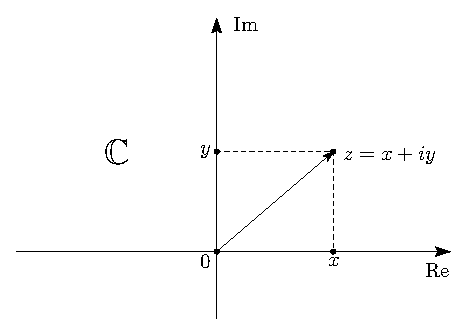
\includegraphics[width=0.45\textwidth]{AL1L13_1.eps}
	\label{AL1L13_1}
	\caption{Комплексная плоскость.}
\end{figure}

Сложение/вычитание комплексных чисел $\Leftrightarrow$ сложение/вычитание соответствующих векторов в комплексной плоскости по правилу параллелограмма.
\begin{figure}[H]
	\centering
	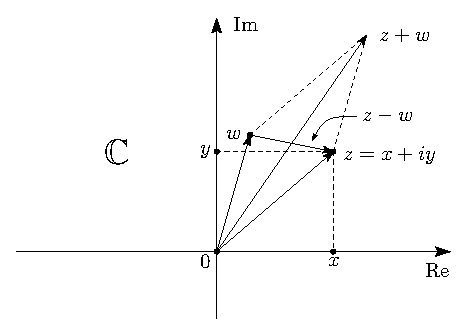
\includegraphics[width=0.45\textwidth]{AL1L13_2.eps}
	\label{AL1L13_2}
	\caption{Векторное сложение/вычитание.}
\end{figure}

Таким образом, операция прибавления комплексного числа (ко всем остальным комплексным числам) это тоже самое что и параллельный перенос на комплексной плоскости, с точки зрения геометрии. 

\begin{defn}
	\uwave{Модулем комплексного числа} $z = x + iy$ называется число $|z| = \sqrt{x^2 + y^2}$.
\end{defn}

С геометрической точки зрения, модуль это расстояние от точки, соответствующей числу $z$ до начала координат или, что тоже самое, длина вектора, задающего комплексное число $z$.


\begin{defn}
	\uwave{Сопряженным комплексным числом} числа $z = x + iy$ называется число $\ovl{z} = x - iy$.
\end{defn}

\begin{figure}[H]
	\centering
	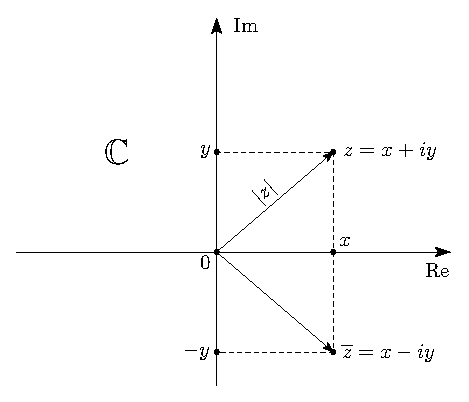
\includegraphics[width=0.45\textwidth]{AL1L13_3.eps}
	\label{AL1L13_3}
	\caption{Модуль числа $z$ и его сопряженное комплексное число.}
\end{figure}

\begin{prop}(\textbf{Свойства сопряженных чисел})
	\begin{enumerate}[label=\arabic*)]
		\item $\ovl{z + w} = \ovl{z} + \ovl{w}$;
		\item $\ovl{z{\cdot}w} = \ovl{z}{\cdot}\ovl{w}$;
		\item $\ovl{z} = z \Leftrightarrow z = \RE(z) \in \MR$;
		\item $z{\cdot}\ovl{z} = |z|^2$;
		\item $\ovl{\ovl{z}} = z$;
		\item $z + \ovl{z} = 2\RE{(z)}$;
		\item $z = -\ovl{z} \Leftrightarrow z = \IM(z) \in \MC$;
	\end{enumerate}
\end{prop}
\begin{proof}\hfill
	\begin{enumerate}[label=\arabic*)]
		\item Пусть $z = x + iy, \, w = u + iv \Rightarrow \ovl{z} = x -iy, \, \ovl{w} = u - iv$, тогда:
		$$
			z+w = (x + u) + i(y + v) \Rightarrow \ovl{z+w} = (x+u) - i(y + v) = x -iy + u - iv = \ovl{z} + \ovl{w}
		$$
		\item Пусть $z = x + iy, \, w = u + iv$, тогда:
		$$
			z{\cdot}w = (x{\cdot}u - y{\cdot}v) + i(x{\cdot}v + y{\cdot}u) \Rightarrow \ovl{z{\cdot}w} = (x{\cdot}u - y{\cdot}v) - i(x{\cdot}v + y{\cdot}u)
		$$
		$$
			\ovl{z}{\cdot}\ovl{w} = (x{\cdot}u - (-y){\cdot}(-v)) + i(x{\cdot}(-v) + u{\cdot}(-y))= (x{\cdot}u - y{\cdot}v) - i(x{\cdot}v + u{\cdot}y)
		$$
		\item Пусть $z = x + iy$, тогда:
		$$
			\ovl{z} = x - iy = z = x + iy \Leftrightarrow y = 0 \Leftrightarrow z = x + i{\cdot}0 = x = \RE(z)\in \MR
		$$
		\item Пусть $z = x + iy \Rightarrow \ovl{z} = x - iy$, тогда:
		$$
			z{\cdot}\ovl{z} = (x + iy){\cdot}(x - iy) = x^2 - i^2{\cdot}y^2 = x^2 + y^2 = |z|^2 
		$$
		\item Пусть $z = x + iy \Rightarrow \ovl{z} = x - iy$, тогда:
		$$
			\ovl{\ovl{z}} = \ovl{x - iy} = x + iy = z
		$$
		\item Пусть $z = x + iy \Rightarrow \ovl{z} = x - iy$, тогда:
		$$
			z + \ovl{z} = x + iy + x - iy = 2x = 2\RE(z)
		$$
		\item Пусть $z = x + iy \Rightarrow \ovl{z} = x - iy$, тогда:
		$$
			z = x + iy = - \ovl{z} = - x + iy \Rightarrow x = - x \Rightarrow  x =0 \Rightarrow z = iy = \IM(z) \in \MC
		$$
	\end{enumerate}
\end{proof}
\begin{rem}
	Свойства $1)$ и $2)$ означают, что операция сопряжения: $z \mapsto \ovl{z}$ является изоморфизмом поля комплексных чисел само с собой: $\MC \xrightarrow[\sim]{} \MC$ (биективность - очевидна по определению сопряжения, согласованность с операциями следует из $1)$ и $2)$).
\end{rem}
\begin{rem}
	Операция сопряжения является \uwave{автоморфизмом} поля $\MC$ в себя.
\end{rem}

\begin{prop}(\textbf{Деление комплексных чисел в алгебраической форме})
	$$
		\forall z,w \in \MC, z \neq 0, \, \dfrac{w}{z} = w{\cdot}z^{-1} = \dfrac{w{\cdot}\ovl{z}}{|z|^2}
	$$
\end{prop}
\begin{proof}
	$$
		\forall z \in \MC, \, z{\cdot}\ovl{z} = |z|^2, \, z \neq 0 \Rightarrow |z| > 0 \Rightarrow z{\cdot}\dfrac{\ovl{z}}{|z|^2} = 1 \Rightarrow z^{-1} = \dfrac{\ovl{z}}{|z|^2} \Rightarrow 
	$$
	$$	
		\Rightarrow \forall z,w \in \MC, z \neq 0, \,  w{\cdot}z^{-1} = \dfrac{w{\cdot}\ovl{z}}{|z|^2}
	$$
\end{proof}

\begin{rem}
	По-другому, можно было показать так:
	$$
		\forall z,w \in \MC, z \neq 0, \,  \dfrac{w}{z} = \dfrac{w{\cdot}\ovl{z}}{z{\cdot}\ovl{z}} = \dfrac{w{\cdot}\ovl{z}}{|z|^2}
	$$
	то есть, если мы хотим поделить одно комплексное число на другое, то надо и числитель, и знаменатель этой дроби умножить на число, сопряженное к знаменателю, тогда в знаменателе появится положительное действительное число, на которое можно отдельно поделить, а в числителе будет произведение, которое мы можем выяснить в алгебраической форме. 
\end{rem}

\end{document}